% !TEX root = ../slides.tex
%
\tikzsetnextfilename{multi-pocket}
%
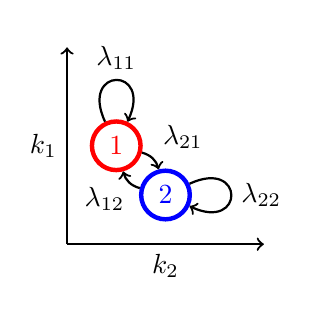
\begin{tikzpicture}[scale=2.5, thick]
    \useasboundingbox (-0.2, -0.2) rectangle (1.1, 1.1);

    \draw [->, thick] (0, 0) -- (0, 1);
    \draw [->, thick] (0, 0) -- (1, 0);

    \node [left]  at (0, 0.5) {$k_1$};
    \node [below] at (0.5, 0) {$k_2$};

    \node [shape=circle, draw, ultra thick, red]  (1) at (0.25, 0.50) {1};
    \node [shape=circle, draw, ultra thick, blue] (2) at (0.50, 0.25) {2};

    \begin{scope}[pos=0.5]
        \draw [->] (1) edge [loop, out=115, in=65, looseness=7]
            node [above] {$\lambda_{1 1}$} (1);
        \draw [->] (1) edge [bend left]
            node [above right] {$\lambda_{2 1}$} (2);
        \draw [->] (2) edge [bend left]
            node [below left=-2pt] {$\lambda_{1 2}$} (1);
        \draw [->] (2) edge [loop, out=25, in=-25, looseness=7]
            node [right] {$\lambda_{2 2}$} (2);
    \end{scope}
\end{tikzpicture}%
